\documentclass[conference]{IEEEtran}
\IEEEoverridecommandlockouts
% The preceding line is only needed to identify funding in the first footnote. If that is unneeded, please comment it out.
\usepackage{cite}
\usepackage{amsmath,amssymb,amsfonts}
\usepackage{algorithmic}
\usepackage{graphicx}
\usepackage{hyperref}
\usepackage{eso-pic}
\usepackage{enumitem}
\usepackage{textcomp}
\usepackage{listings}
\usepackage{xcolor}
\def\BibTeX{{\rm B\kern-.05em{\sc i\kern-.025em b}\kern-.08em
    T\kern-.1667em\lower.7ex\hbox{E}\kern-.125emX}}
\begin{document}

\AddToShipoutPictureBG*{
  \AtPageUpperLeft{
    \hspace{1.5 cm} 
    \raisebox{-4.7 cm}[0pt][0pt]{
      
\includegraphics[width=3.5 cm]{figs/IITH.png}
    }
  }
}

\title{ 
	\textbf{UGV - Toycar}
}
\author{Gajjarapu Satyanarayana \\ AI24BTECH11009}

\maketitle

\tableofcontents

\renewcommand{\thefigure}{\theenumi}
\renewcommand{\thetable}{\theenumi}

\bigskip

\begin{abstract}
Controlling a toycar (UGV) via Bluetooth and Speech.
\end{abstract}


\section{Hardware Setup}
%
\begin{enumerate}[label=\thesection.\arabic*,ref=\thesection.\theenumi]

\item Assemble the chassis, fix the motors and mount the wheels to build the toycar.

\item Fix the breadboard on the base of the toycar.

\item Take an ESP32 module for communication purposes.
\item Plug the \textbf{L293D} motor driver IC in Fig. \ref{fig:l293d_ic} on the breadboard.

\begin{figure}[!ht]
\centering
\resizebox{0.4\textwidth}{!}{%
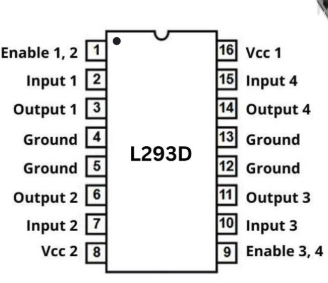
\includegraphics{figs/L293D_IC.png}
}%
\caption{L293D Motor Driver IC}
\label{fig:l293d_ic}
\end{figure}

\item The connections between the L293D output pins and the motors ($M_1, M_2$) are according to Table \ref{table:1}
\begin{table}[h!]
  \centering
  \begin{tabular}[12pt]{ |c| c| c| c| c|}
    \hline
    \textbf{L293D IC} & 3 & 6 & 11 & 14 \\ 
    \hline
    \textbf{Motors} & $M_1$ (+) & $M_1$ (-) & $M_2$ (+) & $M_2$ (-)\\ 
    \hline 
    \end{tabular}

  \caption{L293D \& Motors connections}
  \label{table:1}
\end{table}

\item Connect any 4 GPIO pins (\textbf{Ex}: 25, 26, 33 \& 32) of ESP32 in Fig. \ref{fig:esp32} to L293D inputs
\begin{figure}[!ht]
\centering
\resizebox{0.4\textwidth}{!}{%
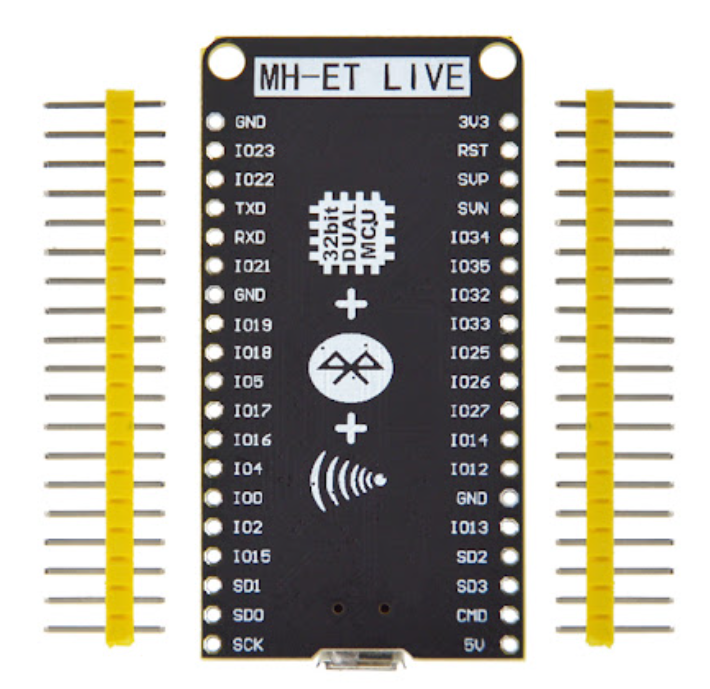
\includegraphics{figs/ESP32.png}
}%
\caption{ESP 32}
\label{fig:esp32}
\end{figure}
\item The connections between the ESP32 and the L293D input pins are according to Table \ref{table:2}
\begin{table}[h!]
  \centering
  \begin{tabular}[12pt]{ |c| c| c| c| c|}
    \hline
    \textbf{ESP32} & 32 & 33 & 25 & 26 \\ 
    \hline
    \textbf{L293D IC} & 3 & 6 & 11 & 14 \\ 
    \hline
    \end{tabular}

  \caption{L293D \& ESP32 connections}
  \label{table:2}
\end{table}

\item Connect the ground pins of the L293D IC and the ESP32 to a common ground on the breadboard.  

\item Connect the 5V pin of the ESP32 to the VCC 1 pin of the L293D IC.  

\end{enumerate}
%
\section{Implementation}

\subsection{Dabble}
\begin{enumerate}[label=\thesection.\arabic*
,ref=\thesection.\theenumi]

\item Install \textbf{Dabble} app using Google Playstore in an Android mobile.

\item Upload the following code to the ESP32 using any IDE.
\fbox{\parbox{\linewidth}{%
wget \url{https://github.com/Satyanarayana-123456/UGV_toycar/blob/main/codes/dabble_gamepad.cpp}%
}}

\item After uploading the above code, plug the ESP32 to a power bank via a micro-USB cable.

\item Open the Dabble app and connect to the ESP32 via bluetooth. The app interface looks like Fig. \ref{fig:dabble_home}
\begin{figure}[!ht]
\centering
\resizebox{0.4\textwidth}{!}{%
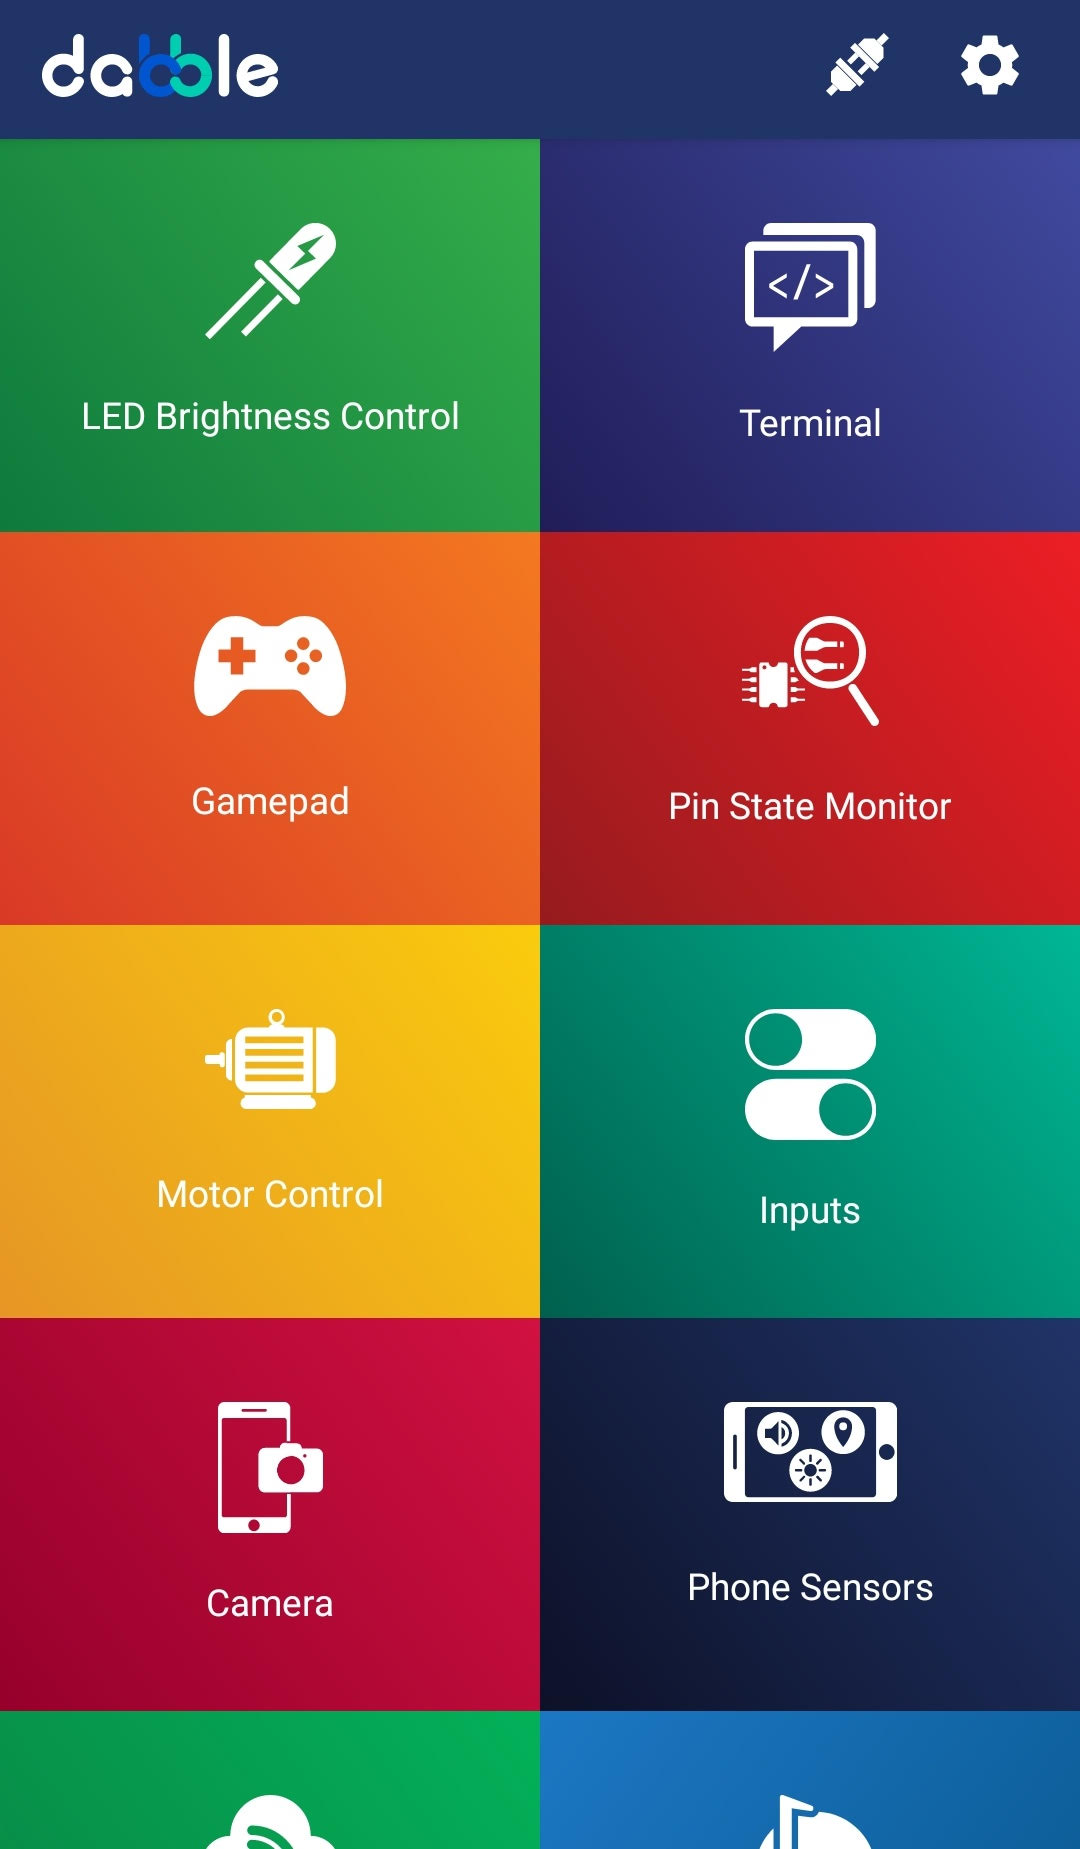
\includegraphics{figs/dabble_home.jpg}
}%
\caption{Dabble Interface}
\label{fig:dabble_home}
\end{figure}

\item Now use the \textbf{Gamepad} of the app in Fig. \ref{fig:dabble_gamepad} to control the toycar.
\begin{figure}[!ht]
\centering
\resizebox{0.5\textwidth}{!}{%
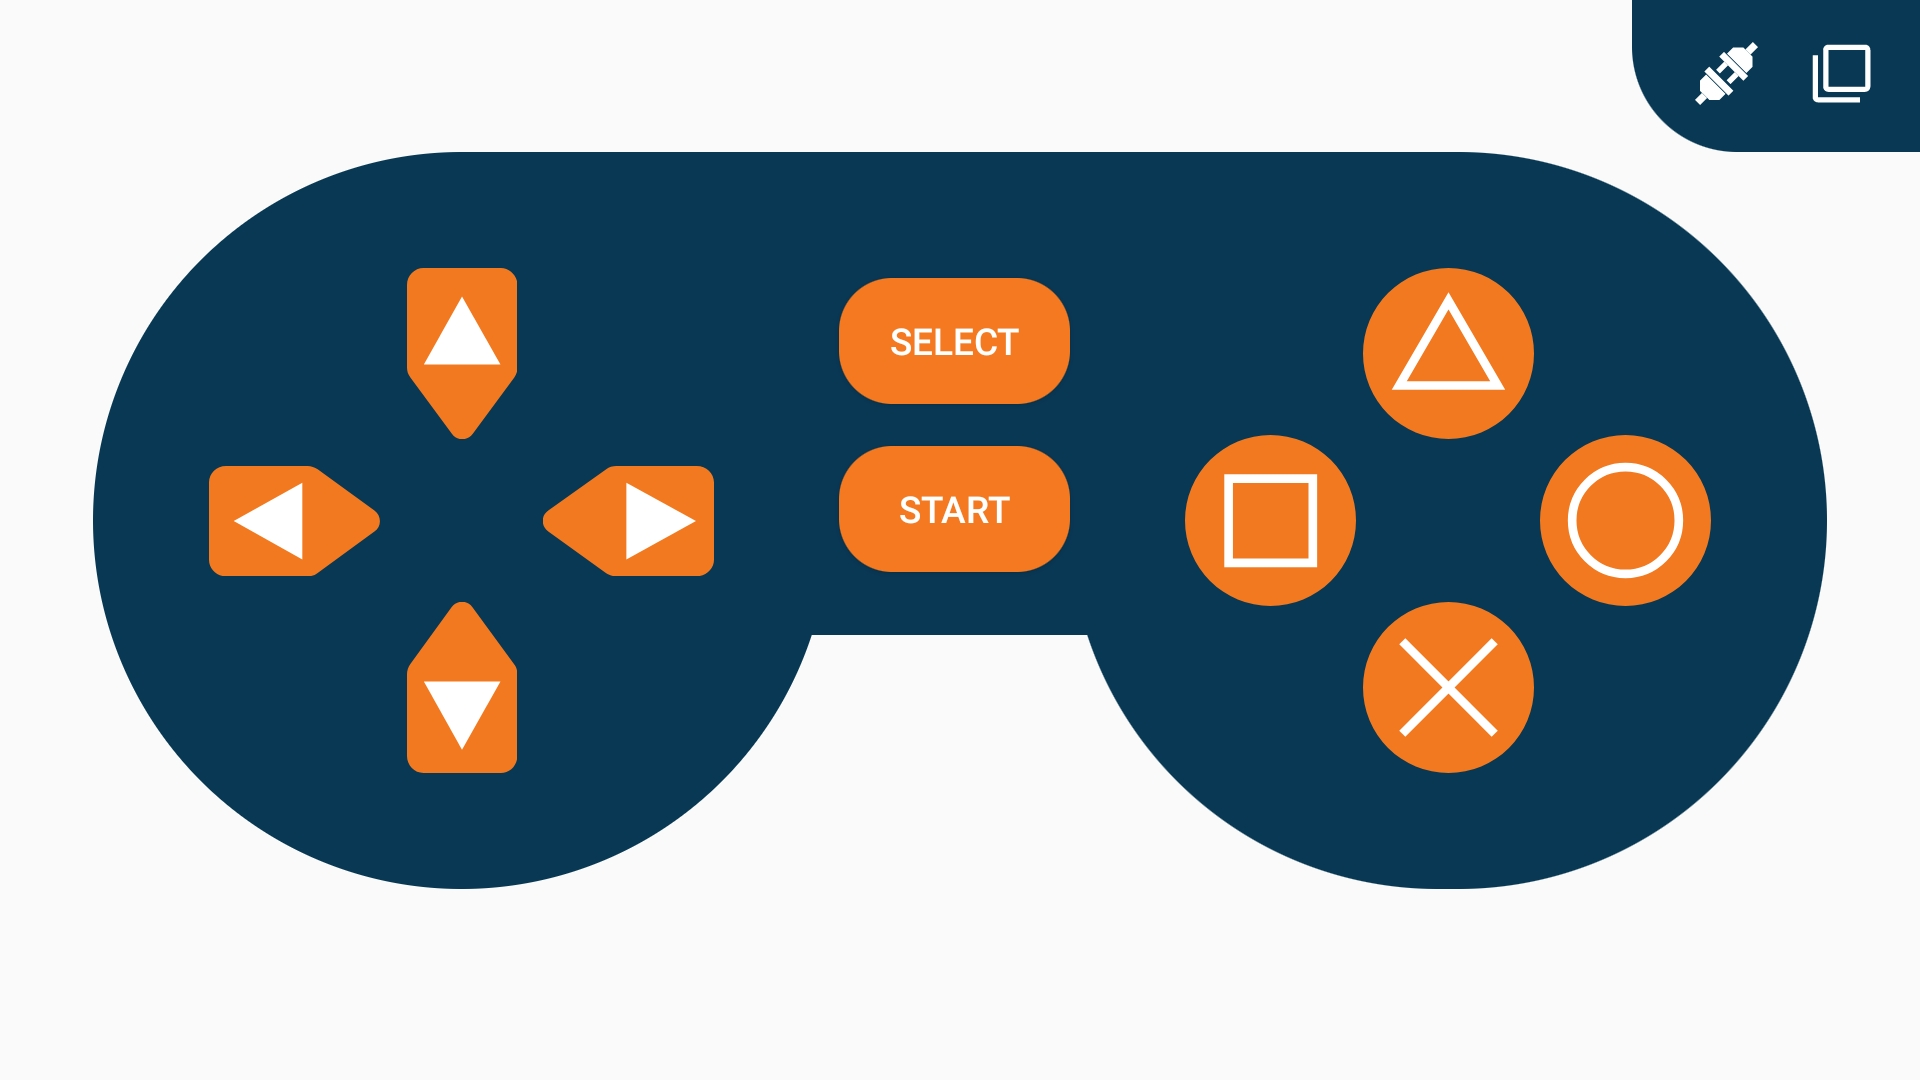
\includegraphics{figs/dabble_gamepad.jpg}
}%
\caption{Gamepad in Dabble App}
\label{fig:dabble_gamepad}
\end{figure}

\item Operate the left-side control buttons labeled \textit{Forward, Back, Left \& Right} to give the respective commands.

\subsection{Arduino Bluetooth Controller}

\item Install \textbf{Arduino Bluetooth Controller} app using Google Playstore in an Android mobile.

\item Upload the following code to the ESP32 using any IDE.
\fbox{\parbox{\linewidth}{%
wget \url{https://github.com/Satyanarayana-123456/UGV_toycar/blob/main/codes/ABC_voice.cpp}%
}}

\item After uploading the above code, plug the ESP32 to a power bank via a micro-USB cable.

\item Open the Arduino Bluetoth Controller app and connect to the ESP32 via bluetooth. The app interface looks like Fig. \ref{fig:ABC_home}

\begin{figure}[!ht]
\centering
\resizebox{0.4\textwidth}{!}{%
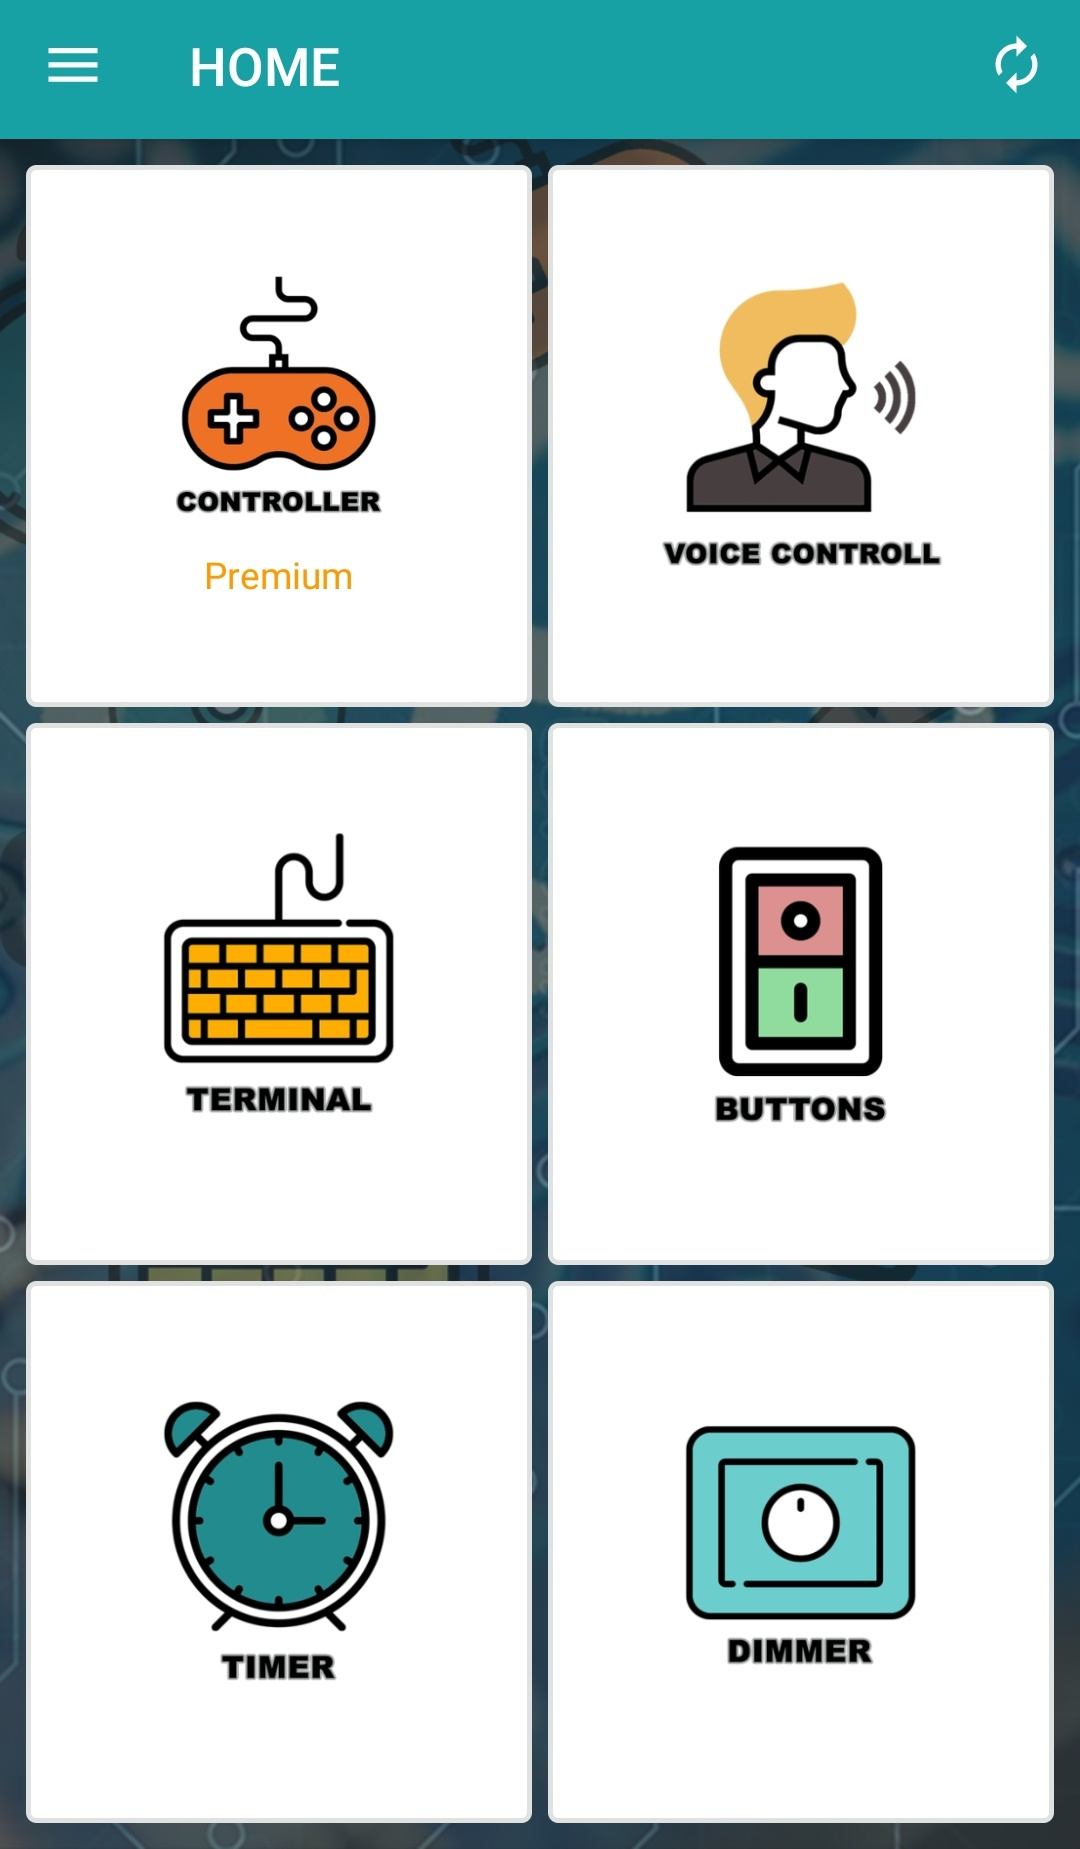
\includegraphics{figs/ABC_home.jpg}
}%
\caption{Arduino Bueetoth Controller Interface}
\label{fig:ABC_home}
\end{figure}

\item Now use the \textbf{Voice Control} section of the app to control the toycar.

\item The commands which the voice control takes are \textit{Left, Right, Forward, Back \& Stop}.

\end{enumerate}
\end{document}
l
